% vim: ts=8 sts=8 sw=4 et tw=75
\chapter{小语言}
\label{chap:little_languages}
\marginpar{131}

人们经常使用 awk 开发 ``小语言'' 的翻译器 (``小语言'' 指的是特定于
某些应用领域的专用编程语言), 
开发翻译器的原因主要有三点. 首先, 它可以帮助你了解语言处理程序的工作流程.
本章的第一个例子是一个汇编程序, 虽然只有 20 来行, 但已经包含了汇编过程
的核心要素, 为了执行汇编程序, 我们还要开发一个解释程序. 汇编程序与
解释程序反映了早期阶段汇编语言与机器架构的关系. 其他例子还包括一个
后缀计算器, 和 awk 子集的递归下降分析器.

第二个原因是在实际工作中, 为了实现一个专用的编程语言, 通常需要投入大
量的精力与财力, 不过在这之前, 我们有必要测试一下新语言的语法和语义. 
作为示例, 本章讨论了一个绘图语言和一个参数设置语言, 后者用于设置排序命令
的参数.

最后一点是希望编程语言能够在实际的工作发挥作用, 就比如说本章所开发的
计算器.

语言处理程序围绕下面这个模型构造而成:
\begin{center}
\begin{tikzpicture}
    \draw[thick]
        (-1.5, 0) -- (-1.5, 1.0) -- (1.5, 1.0) -- (1.5, 0) -- (-1.5, 0);
    \draw[thick]
        (-4.0, 3.0) -- (-4.0, 4.0) -- (-1.0, 4.0) -- (-1.0, 3.0) -- (-4.0,
        3.0);
    \draw[thick]
        (4.0, 3.0) -- (4.0, 4.0) -- (1.0, 4.0) -- (1.0, 3.0) -- (4.0, 3.0);
    
    \draw[thick,->]
        (-6.0, 3.5) -- (-4.0, 3.5);
    \draw[thick,->]
        (-1.0, 3.5) -- (1.0, 3.5);
    \draw[thick,->]
        (4.0, 3.5) -- (6.0, 3.5);
    \draw[thick,<->]
        (-2.0, 3.0) -- (-1.0, 1.0);
    \draw[thick,<->]
        (2.0, 3.0) -- (1.0, 1.0);

    \node[above] at (-5.0, 3.5) {源程序};
    \node at (-2.5, 3.5) {分析器};
    \node at (2.5, 3.5) {合成器};
    \node[above] at (5.0, 3.5) {目标程序};
    \node at (0, 0.5) {符号表};
\end{tikzpicture}
\end{center}

分析器 (analyzer) 是语言处理程序的前端, 它负责读取源程序 (source program)
并将其切分成 一个个词法单元, 词法
单元包括运算符, 操作数等. 分析器对源程序进行语法检查, 如果源程序含有语法
错误, 它就会打印一条错误消息. 最后, 分析器把源程序转换成某种中间形式,
并传递给后端 (合成器), 合成器 (synthesizer) 再根据中间形式生成目标程序
(target program). 合成器在生成
目标程序的过程中需要和符号表 (symbol table) 通信, 而符号表中的内容由分析
器收集而来.
虽然我们把语言的处理过程描述成多个界限分明的不同步骤, 但实际上, 这些界限
通常很模糊, 而且有些步骤有可能被合并成一个.
\marginpar{132}

利用 awk 为实验性语言构造处理程序非常方便, 这是因为它支持许多和语言翻译
相关的操作. 对源程序的分析可以通过字段分割与正则表达式来完成, 用关联数组
管理符号表, 用 \texttt{printf} 生成目标代码.

关于上面提到的几点, 我们将通过开发几个翻译器来进一步说明. 在保证足够说明
问题的前提下,  将尽量保持程序的简短, 而把润色与优化留到习题中.

\section{汇编程序与解释程序}
\label{subsec:an_assembler_and_interpreter}

我们的第一个例子是虚拟计算机的汇编程序, 虚拟计算机这个概念经常出现在
计算机体系 结构或系统编程的基础课程中. 虚拟计算机有一个累加器, 十条
指令, 按字编址且大小为 1000 字的内存, 我们假设内存的一个 ``字'' 可以
保存5个十进制数位, 如果某个字存放的是一条指令, 那么前两个数位表示操作
码, 最后三个数位表示内存地址. 所有的汇编语言指令在表
\ref{tbl:assembly_language_instructions} 中列出.
\begin{figure}[ht]
\captionsetup{type=table}
\caption{汇编语言指令集}
\label{tbl:assembly_language_instructions}
\begin{center}
    \begin{tabular}{c|l|l}
        \hline
        \hline
        \multicolumn{1}{c|}{操作码}          & \multicolumn{1}{c|}{指令}    &
        \multicolumn{1}{c}{意义}  \\
        \hline
        \texttt{01}     & \texttt{get}  & 从输入读取一个数, 并存放到累
        加器中 \\
        \texttt{02}     & \texttt{put}  & 把累加器的值写到输出 \\
        \texttt{03}     & \texttt{ld M}  & 把地址为 \texttt{M} 的内存单元
        的值读取到累加器中 \\
        \texttt{04}     & \texttt{st M}  & 把累加器的值存放到地址为 
        \texttt{M} 的内存单元中 \\
        \texttt{05}     & \texttt{add M} & 把地址为 \texttt{M} 的内存单元 
        的值与累加器的值相加, 再把结果存放到累加器中 \\
        \texttt{06}     & \texttt{sub M} & 把地址为 \texttt{M} 的内存单元 
        的值与累加器的值相减, 再把结果存放到累加器中 \\
        \texttt{07}     & \texttt{jpos M} & 如果累加器的值为正, 则跳转到
        内存地址 \texttt{M} \\
        \texttt{08}     & \texttt{jz M} & 如果累加器的值为零, 则跳转到 
        内存地址 \texttt{M}     \\
        \texttt{09}     & \texttt{j M}  & 跳转到内存地址 \texttt{M} \\
        \texttt{10}     & \texttt{halt} & 停止执行 \\
                        & \texttt{const C} & 伪操作符, 用于定义一个常量
                        \texttt{C} \\
        \hline
    \end{tabular}
\end{center}
\end{figure}

汇编语言程序由语句序列组成, 每一条语句都包括三个部分: 标号, 操作符, 
操作数, 任意一个部分都可以省略, 标号如果存在, 则必须是所在行的第一个
字段. 程序可以包含 awk 形式的注释. 这里有一个简单的汇编语言程序, 它
的功能是输出多个整数的和, \texttt{0} 表示输入结束.
\marginpar{133}
\begin{awkcode}
    # print sum of input numbers (terminated by zero)

         ld    zero   # initialize sum to zero
         st    sum
    loop get          # read a number
         jz    done   # no more input if number is zero
         add   sum    # add in accumulated sum
         st    sum    # store new value back in sum
         j     loop   # go back and read another number

    done ld    sum    # print sum
         put
         halt

    zero const 0
    sum  const
\end{awkcode}

对应的目标程序由整数序列组成, 这些整数其实就是程序的机器码形式, 当目标
程序运行时, CPU 从内存中读取指令, 译码并执行. 上面程序的机器码是:
\begin{awkcode}
     0: 03010           ld      zero    # initialize sum to zero
     1: 04011           st      sum
     2: 01000      loop get             # read a number
     3: 08007           jz      done    # no more input if number is zero
     4: 05011           add     sum     # add in accumulated sum
     5: 04011           st      sum     # store new value back in sum
     6: 09002           j       loop    # go back and read another number
     7: 03011      done ld      sum     # print sum
     8: 02000           put
     9: 10000           halt
    10: 00000      zero const 0
    11: 00000      sum  const
\end{awkcode}
第一个字段是内存地址, 第二个字段是编码后的指令. 内存地址 0 存放的是汇编
语言程序的第一条指令: \texttt{ld zero}.

汇编程序对源程序进行汇编时需要遍历两次. 第一次遍历利用字段分割操作对源
程序进行词法与语法检查: 读取汇编语言源程序, 忽略注释, 为每一个标号分配
内存地址, 把操作符与操作数的中间表示形式写到一个临时文件中. 第二次遍历
读取临时文件, 根据第一次遍历时计算的结果, 把符号化的操作数转换成内存地
址, 对操作符与操作数进行编码, 把最终的机器语言程序保存到数组 \texttt{mem}
中.

我们将会开发一个解释器来完成另一半的工作, 解释器可以用来模拟计算机执行
机器语言程序时所表现出的行为. 解释器循环地从 \texttt{mem} 中读取指令,
把指令译码成操作符与操作数, 再模拟指令的执行. 变量 \texttt{pc} 用来模拟
程序计数器 (program counter).
\marginpar{134}
\begin{awkcode}
    # asm - assembler and interpreter for simple computer
    #   usage: awk -f asm program-file data-files...

    BEGIN {
        srcfile = ARGV[1]
        ARGV[1] = ""  # remaining files are data
        tempfile = "asm.temp"
        n = split("const get put ld st add sub jpos jz j halt", x)
        for (i = 1; i <= n; i++)   # create table of op codes
            op[x[i]] = i-1

    # ASSEMBLER PASS 1
        FS = "[ \t]+"
        while (getline <srcfile > 0) {
            sub(/#.*/, "")         # strip comments
            symtab[$1] = nextmem   # remember label location
            if ($2 != "") {        # save op, addr if present
                print $2 "\t" $3 >tempfile
                nextmem++
            }
        }
        close(tempfile)

    # ASSEMBLER PASS 2
        nextmem = 0
        while (getline <tempfile > 0) {
            if ($2 !~ /^[0-9]*$/)  # if symbolic addr,
                $2 = symtab[$2]    # replace by numeric value
            mem[nextmem++] = 1000 * op[$1] + $2  # pack into word
        }

    # INTERPRETER
        for (pc = 0; pc >= 0; ) {
            addr = mem[pc] % 1000
            code = int(mem[pc++] / 1000)
            if      (code == op["get"])  { getline acc }
            else if (code == op["put"])  { print acc }
            else if (code == op["st"])   { mem[addr] = acc }
            else if (code == op["ld"])   { acc  = mem[addr] }
            else if (code == op["add"])  { acc += mem[addr] }
            else if (code == op["sub"])  { acc -= mem[addr] }
            else if (code == op["jpos"]) { if (acc >  0) pc = addr }
            else if (code == op["jz"])   { if (acc == 0) pc = addr }
            else if (code == op["j"])    { pc = addr }
            else if (code == op["halt"]) { pc = -1 }
            else                         { pc = -1 }
        }
    }
\end{awkcode}

数组 \texttt{symtab} 记录标号的内存地址, 如果当前输入行没有标号, 那么内存
地址赋值给 \texttt{symtab[""]}.

标号是汇编语句的第一个字段, 操作符前面有一个空格符. 第一次遍历前, 把
\marginpar{135}
\texttt{FS} 设置成 \verb'[ \t]+', 于是字段分隔符变成由多个空格符和制表
符组成的序列. 比较特殊的是, 前导空格也被当作字段分隔符, 所以 \verb'$1'
总是标号, 而 \verb'$2' 总是操作符.

因为伪操作符 \texttt{const} 的 ``操作码'' 是 0, 所以在第二次遍历时, 语句
\begin{awkcode}
    mem[nextmem++] = 1000 * op[$1] + $2  # pack into word
\end{awkcode}
可以同时用来存放常数与指令.

\begin{exercise}
    \label{exer:asm}
    修改 \texttt{asm}, 打印程序与内存的内容, 就像上面显示的那样.
\end{exercise}

\begin{exercise}
    增强解释器的功能, 打印指令的执行轨迹.
\end{exercise}

\begin{exercise}
    适当扩大汇编语言的规模, 比如添加错误处理代码与其他条件判断指令. 为了 
    方便用户使用, 你会怎么处理立即数, 比如 \texttt{add = 1} (如果 
    不支持立即数, 就必须要求用户自己创建一个名为 \texttt{one} 的
    内存单元)?
\end{exercise}

\begin{exercise}
    写一个反汇编程序, 把内存中的内容转换成对应的汇编语言.
\end{exercise}

\begin{exercise}
    查看一台真实的机器 (比如 Apple-II 和 Commodore 的 6502 芯片, 或
    IBM PC 及其兼容机的 8086 芯片族), 尝试为它的汇编语言子集写
    一个汇编程序.
\end{exercise}

\section{绘图语言}
\label{sec:a_language_for_drawing_graphs}

利用字段分割操作, 很容易就可以对我们自己定义的汇编语言进行词法和语法分析,
这种简易性对一些高级语言来说同样成立. 我们的下一个例子是 \texttt{graph} 
的语言处理程序, \texttt{graph} 是一种用来画数据坐标图的原型语言. 输入
是一张图的规范说明, 规范说明的每一行都表示一个数据点, 或坐标轴的标签
信息. 数据点有两种表示形式: 一对 \textit{x}-\textit{y}, 或者只有一个
\textit{y}, 此时默认 \textit{x} 是从 1 开始的递增序列, 即 1, 2, 3, 等等.
两种形式中, 数据值的后面都可以跟随一个可选的非数字字符, 作为数据点的
绘图字符 (默认是星号 \verb'*').  标签信息由一个关键词和多个参数值组成:
\begin{pattern}
\indent\texttt{label}\ \textit{caption} \par
\indent\texttt{range}\ \textit{xmin}\ \textit{ymin}\ \textit{xmax}\
    \textit{ymax} \par 
\indent\texttt{left ticks}\ \ \textit{t}$_1$\ \textit{t}$_2$ ... \par 
\indent\texttt{bottom ticks}\ \ \textit{t}$_1$\ \textit{t}$_2$ ... \par 
\indent\texttt{height}\ \textit{number}\par
\indent\texttt{width}\ \textit{number}\par
\end{pattern}
这些行的出现顺序是任意的, 任意一行都可以省略, 也不需要指定数据的值的
范围.

处理程序按比例调整数据点的大小, 并生成绘图命令. 为了使讨论更加具体,
我们把它们打印到 $24 \times 80$ 的字符数组中, 但是, 如果是为某些
图像设备生成绘图命令, 实现起来其实也很容易. 例如, 输入数据:
\marginpar{136}
\begin{awkcode}
    label Annual Traffic Deaths, USA, 1925-1984
    range 1920 5000 1990 60000
    left ticks 10000 30000 50000
    bottom ticks 1930 1940 1950 1960 1970 1980

    1925 21800
    1930 31050
    1935 36369
    ...
    1981 51500
    1982 46000
    1983 44600
    1984 46200
\end{awkcode}
的输出是\footnote{英文原版没有给出完整的统计数据, 下面这张表的统计数据来自
    \url{https://en.wikipedia.org/wiki/List_of_motor_vehicle_deaths_in_U.S._by_year}
 --- 译者注}:
{\footnotesize
\begin{lstlisting}[basicstyle = \ttfamily, lineskip = -2pt]
      |------------------------------------------------------------------------|
      |                                                                        |
      |                                                  *  **                 |
      |                                               * * **        **         |
50000 -                                                *          *   *        |
      |                                             **           *             |
      |                                                       ***      * *     |
      |                                            *                    *      |
      |                                     *     *                            |
      |                               ***  * *****                             |
      |               *    *         *   *                                     |
30000 -         *                ****                                          |
      |                                                                        |
      |                         *                                              |
      |                                                                        |
      |    *                                                                   |
      |                                                                        |
      |                                                                        |
      |                                                                        |
10000 -                                                                        |
      |                                                                        |
      |---------|----------|---------|----------|---------|----------|---------|
               1930       1940      1950       1960      1970       1980        
                        Annual Traffic Deaths, USA, 1925-1984                   
\end{lstlisting}
}

\texttt{graph} 的处理程序分为两个阶段. 主循环读取并解析图的规范说明, 
使用模式辨认不同类型的语句. 图的中间表示形式存放在若干个数组与变量中,
如果必要的话, \texttt{END} 据此计算值的范围, 然后开始绘制边框, 刻度,
标签和数据点. 输出操作被分散在若干个函数中, 这样的话, 即使以后要为
特定的设备对代码进行修改, 也可以把修改局限在小范围内.

到目前为止, 这是我们看过的最长的 awk 程序, 大约有 100 行, 其实它是本书
第二长的程序. 不过不要担心, 程序把一个大任务分成若干个小步骤来完成, 
所以每个部分都很简短.
\marginpar{137}
\begin{awkcode}
    # graph - processor for a graph-drawing language
    #   input:  data and specification of a graph
    #   output: data plotted in specified area

    BEGIN {                # set frame dimensions...
        ht = 24; wid = 80  # height and width
        ox = 6; oy = 2     # offset for x and y axes
        number = "^[-+]?([0-9]+[.]?[0-9]*|[.][0-9]+)" \
                                "([eE][-+]?[0-9]+)?$"
    }
    $1 == "label" {                       # for bottom
        sub(/^ *label */, "")
        botlab = $0
        next
    }
    $1 == "bottom" && $2 == "ticks" {     # ticks for x-axis
        for (i = 3; i <= NF; i++) bticks[++nb] = $i
        next
    }
    $1 == "left" && $2 == "ticks" {       # ticks for y-axis
        for (i = 3; i <= NF; i++) lticks[++nl] = $i
        next
    }
    $1 == "range" {                       # xmin ymin xmax ymax
        xmin = $2; ymin = $3; xmax = $4; ymax = $5
        next
    }
    $1 == "height" { ht = $2; next }
    $1 == "width"  { wid = $2; next }
    $1 ~ number && $2 ~ number {          # pair of numbers
        nd++    # count number of data points
        x[nd] = $1; y[nd] = $2
        ch[nd] = $3    # optional plotting character
        next
    }
    $1 ~ number && $2 !~ number {         # single number
        nd++    # count number of data points
        x[nd] = nd; y[nd] = $1; ch[nd] = $2
        next
    }
    END {    # draw graph
        if (xmin == "") {         # no range was given
            xmin = xmax = x[1]    # so compute it
            ymin = ymax = y[1]
            for (i = 2; i <= nd; i++) {
                if (x[i] < xmin) xmin = x[i]
                if (x[i] > xmax) xmax = x[i]
                if (y[i] < ymin) ymin = y[i]
                if (y[i] > ymax) ymax = y[i]
            }
        }
        frame(); ticks(); label(); data(); draw()
    }
\end{awkcode}
\marginpar{138}
\begin{awkcode}
    function frame() {        # create frame for graph
        for (i = ox; i < wid; i++) plot(i, oy, "-")     # bottom
        for (i = ox; i < wid; i++) plot(i, ht-1, "-")   # top
        for (i = oy; i < ht; i++) plot(ox, i, "|")      # left
        for (i = oy; i < ht; i++) plot(wid-1, i, "|")   # right
    }
    function ticks(    i) {   # create tick marks for both axes
        for (i = 1; i <= nb; i++) {
            plot(xscale(bticks[i]), oy, "|")
            splot(xscale(bticks[i])-1, 1, bticks[i])
        }
        for (i = 1; i <= nl; i++) {
            plot(ox, yscale(lticks[i]), "-")
            splot(0, yscale(lticks[i]), lticks[i])
        }
    }
    function label() {        # center label under x-axis
        splot(int((wid + ox - length(botlab))/2), 0, botlab)
    }
    function data(    i) {    # create data points
        for (i = 1; i <= nd; i++)
            plot(xscale(x[i]),yscale(y[i]),ch[i]=="" ? "*" : ch[i])
    }
    function draw(    i, j) { # print graph from array
        for (i = ht-1; i >= 0; i--) {
            for (j = 0; j < wid; j++)
                printf((j,i) in array ? array[j,i] : " ")
            printf("\n")
        }
    }
    function xscale(x) {      # scale x-value
        return int((x-xmin)/(xmax-xmin) * (wid-1-ox) + ox + 0.5)
    }
    function yscale(y) {      # scale y-value
        return int((y-ymin)/(ymax-ymin) * (ht-1-oy) + oy + 0.5)
    }
    function plot(x, y, c) {  # put character c in array
        array[x,y] = c
    }
    function splot(x, y, s,    i, n) { # put string s in array
        n = length(s)
        for (i = 0; i < n; i++)
            array[x+i, y] = substr(s, i+1, 1)
    }
\end{awkcode}

Awk 很适合处理面向模式的 \texttt{graph} 语言, 之所以这样说是因为它的
规范说明语句是带有值的关键词. 使用这种风格来设计语言是一个很好的
开始: 既方便用户使用, 也方便处理.

\texttt{graph} 是坐标绘图语言 \texttt{grap} 的简化版本, 而 \texttt{grap}
是绘图语言 \texttt{pic} 的预处理器. 
\marginpar{139} 当同时使用 \texttt{grap}, \texttt{pic} 与 \texttt{troff}
时, 同样的数据与几乎相同的描述可以生成下面这张图片:
% 生成 traffic_deaths.eps 的 grap 代码是 (未显示的数据用 ... 表示):
%.G1
%label bottom "Annual Traffic Deaths, USA, 1925-1984"
%coord x 1920,1990 y 5000, 60000
%ticks left out 0.08 from 10000 to 50000 by 20000
%ticks bot out 0.08 from 1930 to 1980 by 10
%
%1925 20771
%1930 31204
%1935 34494
%...
%1983 42589
%1984 44257
%.G2
\begin{center}
    \includegraphics{./images/traffic_deaths.eps}
\end{center}

Awk 很适合用来设计与测验小语言, 如果设计被证明是合理的, 那么就可以用更
高效的语言 (比如 C) 来实现一个产品化的版本. 在某些情况下, 即使是一个
原型产品也可以用在实际生产中, 典型的例子包括对已有工具的定制或包装.

一个特定的实例是定制图表的准备, 在这个实例中, 我们把一门简单的语言, 用
awk 程序转换成 \texttt{grap} 命令. 其他例子还包括散点矩阵 (scatter-plot
matrices), 点阵图 (dotchart, 直方图的一种), 箱线图 (boxplot, 显示了某
个观测集的期望值 (mean) , 四分位数 (quartile) 和 极值 (extreme)) 以及
饼图.

\begin{exercise}
    \label{exer:zhuangzhi}
    修改 \texttt{graph}: 对图进行转置, 即 \textit{x} 轴在垂直方向上,
    而 \textit{y} 轴在水平方向上, 而且可以指定是否以对数的方式显示
    \textit{x} 坐标或 \textit{y} 坐标.
\end{exercise}

\begin{exercise}
    为 \texttt{graph} 添加一条命令, 这条命令可以让 \texttt{graph} 从
    文件中读取数据.
\end{exercise}

\begin{exercise}
    自动计算刻度的位置. (即使最终的实现要用到另一种语言, 但 awk 仍然
    很适合于对算法进行测验)
\end{exercise}

\begin{exercise}
    如果你的系统提供了图形库, 修改 \texttt{graph}, 为图形库生成命令.
    (这是一个对已有工具进行再包装的例子)
\end{exercise}

\marginpar{140}
\section{\textbf{\texttt{sort}} 生成器}
\label{sec:a_sort_generator}

\cterm{如果} 用户知道如何使用 Unix 命令 \texttt{sort} 的话, 那么它将会是
一个非常强大的工具. 但是要记住它所有的选项是非常困难的, 而且对于 ``字段
编号从零开始'' 这个事实, 你可能会觉得不太习惯. 作为小语言的另一个训练,
我们将开发一个 \texttt{sortgen} 程序, 它根据 由自然语言描述的规范说明
来生成排序命令. \texttt{sortgen} 生成排序命令但并不执行 --- 这个工作留
给用户, 因为用户在执行之前可能想要检查一下生成的命令.

\texttt{sortgen} 的输入是一连串的单词或短语, 它们描述了有关排序的选项,
比如字段分隔符, 排序键, 比较的方向或类型. 程序的目标是在尽可能宽松的
语法规则下, 解决比较常见的情况, 比如输入
\begin{awkcode}
    descending numeric order
\end{awkcode}
的输出是
\begin{awkcode}
    sort -rn
\end{awkcode}
更复杂的一个输入是
\begin{awkcode}
    field separator is :
    primary key is field 1
        increasing alphabetic
    secondary key is field 5
        reverse numeric
\end{awkcode}
\texttt{sortgen} 产出的 \texttt{sort} 命令及其选项与第
\ref{chap:reports_and_databases} 章的第一个 \texttt{sort} 命令等价:
\begin{awkcode}
    sort -t':' +0 -1 +4rn -5
\end{awkcode}

\texttt{sortgen} 的核心是一套规则集, 该规则集把单词与短语描述的排序
选项翻译成对应的 \texttt{sort} 命令行选项. 规则集通过 \patact 语句
实现, 模式用于匹配选项的描述字符串, 而动作则计算相应的命令行选项. 比如,
只要选项描述字符串中出现了 ``unique'' 或 ``discard identical'', 就把它
们当作选项 \texttt{-u}, 这个选项的功能是忽略重复条目. 类似的, 字段分隔符
假设是制表符, 可是如果描述中出现了 ``separate'' 这样的字眼, 那就把字
段分隔符设置成对应的单个字符.

最难的部分是多个排序键的处理, 每一个排序键都可以跨越多个字段. 识别
排序键的关键词是 ``key''. 如果描述中出现了这个词, 那么就把一个或两个
互相隔离的数字收集起来当作字段编号. ``key'' 的每一次出现都会为新
的排序键收集选项. 排序键私有的选项包括空格抑制 (\texttt{-b}),
字典序 (\texttt{-d}), 忽略大小写 (\texttt{-f}), 数字序 (\texttt{-n}),
和逆序 (\texttt{-r}).
\marginpar{141}
\begin{awkcode}
    # sortgen - generate sort command
    #   input:  sequence of lines describing sorting options
    #   output: Unix sort command with appropriate arguments

    BEGIN { key = 0 }

    /no |not |n't / { print "error: can't do negatives:", $0; ok = 0 }

    # rules for global options
            { ok = 0 }
    /uniq|discard.*(iden|dupl)/  { uniq = " -u"; ok = 1 }
    /separ.*tab|tab.*sep/        { sep = "t'\t'"; ok = 1 }
    /separ/ { for (i = 1; i <= NF; i++)
                  if (length($i) == 1)
                      sep = "t'" $i "'"
              ok = 1
            }
    /key/   { key++; dokey(); ok = 1 } # new key; must come in order

    # rules for each key

    /dict/                            { dict[key] = "d"; ok = 1 }
    /ignore.*(space|blank)/           { blank[key] = "b"; ok = 1 }
    /fold|case/                       { fold[key] = "f"; ok = 1 }
    /num/                             { num[key] = "n"; ok = 1 }
    /rev|descend|decreas|down|oppos/  { rev[key] = "r"; ok = 1 }
    /forward|ascend|increas|up|alpha/ { next }    # this is sort's default
    !ok   { print "error: can't understand:", $0 }

    END {                        # print flags for each key
        cmd = "sort" uniq
        flag = dict[0] blank[0] fold[0] rev[0] num[0] sep
        if (flag) cmd = cmd " -" flag
        for (i = 1; i <= key; i++)
            if (pos[i] != "") {
                flag = pos[i] dict[i] blank[i] fold[i] rev[i] num[i]
                if (flag) cmd = cmd " +" flag
                if (pos2[i]) cmd = cmd " -" pos2[i]
            }
        print cmd
    }

    function dokey(    i) {      # determine position of key
        for (i = 1; i <= NF; i++)
            if ($i ~ /^[0-9]+$/) {
                pos[key] = $i - 1    # sort uses 0-origin
                break
            }
        for (i++; i <= NF; i++)
            if ($i ~ /^[0-9]+$/) {
                pos2[key] = $i
                break
            }
        if (pos[key] == "")
            printf("error: invalid key specification: %s\n", $0)
        if (pos2[key] == "")
            pos2[key] = pos[key] + 1
    }
\end{awkcode}

\marginpar{142}
为了避免处理类似于 ``don't discard duplicates'' 或 ``no numeric data'' 
这样的输入, \texttt{sortgen} 会拒绝含有否定短语的行, 接下来的规则处理
全局选项, 然后是针对当前排序键的选项, 如果程序无法理解某一行的意思,
就会向用户打印一条消息.

这个程序虽然不够聪明, 但是, 如果用户想要用它来获取正确的答案, 而不是
诱导它犯错, 那么\texttt{sortgen} 仍然是一个很有用的工具.

\begin{exercise}
    实现一个新版的 \texttt{sortgen}, 它提供了访问 \texttt{sort} 全部功能
    的方法, 要求程序能够检测出不一致的请求, 比如同时按照字典序与数值对
    数据进行排序.
\end{exercise}

\begin{exercise}
    在对输入语言规范性不作过多要求的前提下, 如何提高 \texttt{sortgen} 
    的精确度.
\end{exercise}

\begin{exercise}
    写一个程序, 把一个排序命令翻译成对应的英文句子, 然后再把句子作
    为 \texttt{sortgen} 的输入.
\end{exercise}

\section{逆波兰式计算器}
\label{sec:a_reverse_polish_calculator}

假设我们现在想要一个计算器, 用来结算支票或计算数学表达式的值. Awk 本身
很适合处理这种计算工作, 但是每次程序发生变化时, 都必须重新运行.
我们需要的是一个随着表达式的输入, 可以自动读取并运算的计算器程序.

为了避免开发语法解析器, 我们要求用户按照逆波兰表示法输入表达式. (``逆''
指的是运算符跟在操作数的后面, ``波兰'' 是因为这种表示法是波兰数学家
Jan Lukasiewicz 发明的). 中缀表达式
\begin{awkcode}
    (1 + 2) * (3 - 4) / 5
\end{awkcode}
写成逆波兰表示法变成
\begin{awkcode}
    1 2 + 3 4 - * 5 /
\end{awkcode}
逆波兰式不需要括号 --- 如果提前知道运算符的操作数个数, 那么表达式就不会
有歧义. 逆波兰式非常适合用栈处理, 由于这个特点, 许多编程语言 (包括
Forth 和 Postscript) 和便捷计算器都把它作为基本表示法来使用.

我们的第一个计算器只能用来计算采用逆波兰式表示法表示的数学表达式,
所有的运算符与操作数都用空格分开. 如果某个字段是操作数, 就把它入栈;
如果是运算符, 就对栈顶的操作数执行对应的运算. 每当一个输入行结束时,
打印栈顶元素的值, 并把它弹出.
\marginpar{143}
\begin{awkcode}
    # calc1 - reverse-Polish calculator, version 1
    #   input:  arithmetic expressions in reverse Polish
    #   output: values of expressions

    {   for (i = 1; i <= NF; i++)
            if ($i ~ /^[+-]?([0-9]+[.]?[0-9]*|[.][0-9]+)$/) {
                stack[++top] = $i
            } else if ($i == "+" && top > 1) {
                stack[top-1] += stack[top]; top--
            } else if ($i == "-" && top > 1) {
                stack[top-1] -= stack[top]; top--
            } else if ($i == "*" && top > 1) {
                stack[top-1] *= stack[top]; top--
            } else if ($i == "/" && top > 1) {
                stack[top-1] /= stack[top]; top--
            } else if ($i == "^" && top > 1) {
                stack[top-1] ^= stack[top]; top--
            } else {
                printf("error: cannot evaluate %s\n", $i)
                top = 0
                next
            }
        if (top == 1)
            printf("\t%.8g\n", stack[top--])
        else if (top > 1) {
            printf("error: too many operands\n")
            top = 0
        }
    }
\end{awkcode}
对于输入 
\begin{awkcode}
    1 2 + 3 4 - * 5 /
\end{awkcode}
\texttt{calc1} 给出的答案是 \texttt{-0.6}.

我们的第二个逆波兰式计算器支持用户自定义变量, 并且可以调用数学函数.
变量名由字母开始, 后跟字母或数字, 语句 \textit{var}\texttt{=} 表示把
栈顶元素弹出, 并赋值给变量 \textit{var}. 如果输入行以赋值语句结束, 
则不会打印出任何值. 一个典型的交互过程看起来就像这样 (由程序打印的内容
向右缩进):
\begin{awkcode}
    0 -1 atan2 pi=
    pi 
        3.1415927
    355 113 / x= x
        3.1415929
    x pi /
        1.0000001
    2 sqrt 
        1.4142136
\end{awkcode}
直接对前一个程序进行扩展, 就可以得到新版的计算器:
\marginpar{144}
\begin{awkcode}
    # calc2 - reverse-Polish calculator, version 2
    #     input:  expressions in reverse Polish
    #     output: value of each expression

    { for (i = 1; i <= NF; i++)
          if ($i ~ /^[+-]?([0-9]+[.]?[0-9]*|[.][0-9]+)$/) {
              stack[++top] = $i
          } else if ($i == "+" && top > 1) {
              stack[top-1] += stack[top]; top--
          } else if ($i == "-" && top > 1) {
              stack[top-1] -= stack[top]; top--
          } else if ($i == "*" && top > 1) {
              stack[top-1] *= stack[top]; top--
          } else if ($i == "/" && top > 1) {
              stack[top-1] /= stack[top]; top--
          } else if ($i == "^" && top > 1) {
              stack[top-1] ^= stack[top]; top--
          } else if ($i == "sin" && top > 0) {
              stack[top] = sin(stack[top])
          } else if ($i == "cos" && top > 0) {
              stack[top] = cos(stack[top])
          } else if ($i == "atan2" && top > 1) {
              stack[top-1] = atan2(stack[top-1],stack[top]); top--
          } else if ($i == "log" && top > 0) {
              stack[top] = log(stack[top])
          } else if ($i == "exp" && top > 0) {
              stack[top] = exp(stack[top])
          } else if ($i == "sqrt" && top > 0) {
              stack[top] = sqrt(stack[top])
          } else if ($i == "int" && top > 0) {
              stack[top] = int(stack[top])
          } else if ($i in vars) {
              stack[++top] = vars[$i]
          } else if ($i ~ /^[a-zA-Z][a-zA-Z0-9]*=$/ && top > 0) {
              vars[substr($i, 1, length($i)-1)] = stack[top--]
          } else {
              printf("error: cannot evaluate %s\n", $i)
              top = 0
              next
          }
      if (top == 1 && $NF !~ /\=$/)
          printf("\t%.8g\n", stack[top--])
      else if (top > 1) {
          printf("error: too many operands\n")
          top = 0
      }
    }
\end{awkcode}

\begin{exercise}
    \label{exer:calc2}
    为 \texttt{calc2} 的标准值 (例如 $\pi$ 与 $\mathrm{e}$) 添加内建变量.
    添加 一个内建变量, 用来表示最后一个输入行的运算结果. 添加两个栈操作
    运算符, 分别用来完成栈顶元素的复制, 与交换栈顶的两个元素.
\end{exercise}

\marginpar{145}
\section{中缀计算器}
\label{sec:an_infix_calculator}

到目前为止, 本章所介绍的语言都拥有易于分析的语法规则. 然而, 大多数高级
语言拥有大量不同优先级的运算符, 嵌套结构 (比如括号与 if-then-else 语句),
以及其他复杂的构造, 所有的这些都要求更强大的解析技术, 而不仅仅是字段
分割与正则表达式匹配. 使用 awk 处理高级语言是可能的, 只要有一个完全
成熟的解析程序即可, 而解析程序可以用任何一种语言来写.
本节将开发一个对数学表达式进行求值的程序, 表达式使用人们通常所熟悉的中
缀表示法表示. 以该程序为先导, 我们会在下一节开发一个更加复杂的
解析程序.

带有运算符 \verb'+', \verb'-', \verb'*' 和 \verb'/' 的数学表达式语法,
可以用我们在第 \ref{chap:processing_words} 章讲过的方法来描述:
\begin{tabbing}
\indent\textit{expr}\hspace{2em}\=$\to$\hspace{2em}\=\textit{term} \\
\indent\> \> \textit{expr}\ \verb'+'\ \textit{term} \\
\indent\> \> \textit{expr}\ \verb'-'\ \textit{term} \\
\indent\textit{term} \> $\to$ \> \textit{factor} \\
\indent\> \> \textit{term}\ \verb'*'\ \textit{factor} \\
\indent\> \> \textit{term}\ \verb'/'\ \textit{factor} \\
\indent\textit{factor}\>$\to$\>\textit{number} \\
\indent\> \> \verb'('\ \textit{expr}\ \verb')'
\end{tabbing}

该语法规则不仅描述了数学表达式的有效形式, 还规定了运算符的优先级和结合
性. 例如, 一个 \textit{expr} 是多个 \textit{term} 的和或差, 而一个 
\textit{term} 由多个 \textit{factor} 组成, 这确保了乘除在加减之前完成.

我们可以把解析过程画成一张语句图来帮助理解, 这与第
\ref{chap:processing_words} 章所描述的生成过程刚好相反. 比如, 表达式 
\texttt{1 + 2 * 3} 的解析过程是:
\begin{center}
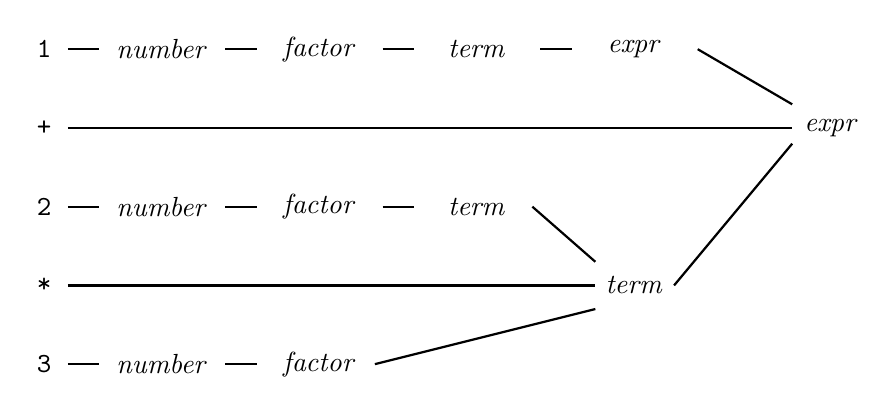
\begin{tikzpicture}
    \node at (0, 0) {\texttt{3}};
    \node at (0, 1) {\texttt{*}};
    \node at (0, 2) {\texttt{2}};
    \node at (0, 3) {\texttt{+}};
    \node at (0, 4) {\texttt{1}};

    \node at (1.5, 0) {\textit{number}};
    \node at (1.5, 2) {\textit{number}};
    \node at (1.5, 4) {\textit{number}};
    \node at (3.5, 0) {\textit{factor}};
    \node at (3.5, 2) {\textit{factor}};
    \node at (3.5, 4) {\textit{factor}};
    \node at (5.5, 2) {\textit{term}};
    \node at (5.5, 4) {\textit{term}};
    \node at (7.5, 4) {\textit{expr}};

    \draw[thick] (0.3, 0) -- (0.7, 0);
    \draw[thick] (2.3, 0) -- (2.7, 0);
    \draw[thick] (0.3, 2) -- (0.7, 2);
    \draw[thick] (2.3, 2) -- (2.7, 2);
    \draw[thick] (4.3, 2) -- (4.7, 2);
    \draw[thick] (0.3, 4) -- (0.7, 4);
    \draw[thick] (2.3, 4) -- (2.7, 4);
    \draw[thick] (4.3, 4) -- (4.7, 4);
    \draw[thick] (6.3, 4) -- (6.7, 4);

    \draw[thick] (0.3, 1) -- (7.0, 1);
    \draw[thick] (6.2, 2.0) -- (7.0, 1.3);
    \draw[thick] (4.2, 0.0) -- (7.0, 0.7);
    \node at (7.5, 1) {\textit{term}};

    \draw[thick] (8.3, 4) -- (9.5, 3.3);
    \draw[thick] (0.3, 3) -- (9.5, 3);
    \node at (10.0, 3) {\textit{expr}};
    \draw[thick] (8.0, 1) -- (9.5, 2.8);
\end{tikzpicture}
\end{center}

为了开发中缀计算器, 我们需要一个表达式解析程序. 只需要多花点精力, 
就可以利用语法规则来构造解析器, 除此之外, 它还可以用来组织程序.
为每一个非终结符写一个函数: 程序使用函数 \texttt{expr}
处理由加号或减号分隔的 \textit{term}, 使用函数 \texttt{term} 处理
由乘号或除号分隔的 \textit{factor}, 最后, 使用函数 \texttt{factor} 来
识别数字和被括号包围起来的 \textit{expr}.

在下面的程序里, 每一个输入行都被当作一个单独的表达式, 表达式被求值并打印
出来.\marginpar{146}
我们仍然要求所有的运算符, 操作数和括号都用空格分开. 变量 \texttt{f} 指向
下一个待检验的字段 (运算符或操作数).
\begin{awkcode}
    # calc3 - infix calculator

    NF > 0 {
        f = 1
        e = expr()
        if (f <= NF) printf("error at %s\n", $f)
        else printf("\t%.8g\n", e)
    }

    function expr(  e) {        # term | term [+-] term
        e = term()
        while ($f == "+" || $f == "-")
            e = $(f++) == "+" ? e + term() : e - term()
        return e
    }

    function term(  e) {        # factor | factor [*/] factor
        e = factor()
        while ($f == "*" || $f == "/")
            e = $(f++) == "*" ? e * factor() : e / factor()
        return e
    }

    function factor(  e) {      # number | (expr)
        if ($f ~ /^[+-]?([0-9]+[.]?[0-9]*|[.][0-9]+)$/) {
            return $(f++)
        } else if ($f == "(") {
            f++
            e = expr()
            if ($(f++) != ")")
                printf("error: missing ) at %s\n", $f)
            return e
        } else {
            printf("error: expected number or ( at %s\n", $f)
            return 0
        }
    }
\end{awkcode}
表达式 \verb'$(f++)' 先取 \verb'$f' 的值, 然后再递增 \texttt{f}, 请注意
它与 \verb'$f++' 的区别, 后者是递增 \verb'$f' 的值.

\begin{exercise}
    构造一组测试集, 对 \texttt{calc3} 进行详尽地测试.
\end{exercise}

\begin{exercise}
    为中缀计算器添加指数运算, 内建函数和变量. 与逆波兰式计算器的实现
    作比较.
\end{exercise}

\begin{exercise}
    加强 \texttt{calc3} 的错误处理功能.
\end{exercise}
\marginpar{147}
\section{递归下降语法分析}
\label{sec:recursive_descent_parsing}

在这一节, 我们为 awk 的子集开发一个递归下降翻译器, 开发语言还是用 awk.
其中处理算术表达式的部分和我们在上一节里展示的程序, 在本质上是一样的.
为了增加真实性, 翻译器将会生成 C 程序, 原来代码中的 awk 运算符用函数
调用来替换. 这个程序在一定程度上说明了语法制导翻译的原理, 以及生成
C 版本 awk 程序的一种方式, C 程序运行起来更快, 也很容易扩展.
基本思路是用函数调用替换掉每一个算术运算符, 比如, \texttt{x=y} 变成
\texttt{assign(x,y)}, \texttt{x+y} 变成 \texttt{eval("+",x,y)}. 主输入
循环用 \texttt{while} 来表示, 每次循环都会调用 \texttt{getrec} 来读取
输入行, 并把输入行分割成字段. 于是, 由
\begin{awkcode}
    BEGIN   { x = 0; y = 1 }

    $1 > x  { if (x == y+1) {
                  x = 1
                  y = x * 2
              } else
                  print x, z[x]
            }

    NR > 1  { print $1 }

    END     { print NR }
\end{awkcode}
得到的 C 代码是
\begin{awkcode}
    assign(x, num((float)0));
    assign(y, num((float)1));
    while (getrec()) {
            if (eval(">", field(num((float)1)), x)) {
                    if (eval("==", x, eval("+", y, num((float)1)))) {
                            assign(x, num((float)1));
                            assign(y, eval("*", x, num((float)2)));
                    } else {
                            print(x, array(z, x));
                    }
            }
            if (eval(">", NR, num((float)1))) {
                    print(field(num((float)1)));
            }
    }
    print(NR);
\end{awkcode}

如果要为某个语言处理程序设计前端, 一个比较好的开始方式是为输入语言写
一套语法规则. 利用 \ref{sec:random_text_generation} 节介绍的表示法,
我们可以这样描述 awk 子集的语法规则:
\marginpar{148}
\begin{tabbing}
    \hspace{4em}
    \textit{program}\hspace{2em}\=$\to$\hspace{2em}\=\textit{opt-begin pa-stats
    opt-end}\\
    \hspace{4em}
    \textit{opt-begin}\>$\to$\>\texttt{BEGIN}\ \textit{statlist}\ |\ 
    \texttt{""}\\
    \hspace{4em}
    \textit{opt-end}\>$\to$\>\texttt{END}\ \textit{statlist}\ |\ 
    \texttt{""}\\
    \hspace{4em}
    \textit{pa-stats}\>$\to$\>\textit{statlist}\ |\ \textit{pattern}\ |\ 
    \textit{pattern statlist} \\
    \hspace{4em}
    \textit{pattern}\>$\to$\>\textit{expr}\\
    \hspace{4em}
    \textit{statlist}\>$\to$\>\verb'{'\ \textit{stats}\ \verb'}'\\
    \hspace{4em}
    \textit{stats}\>$\to$\>\textit{stat stats}\ |\ \texttt{""}\\
    \hspace{4em}
    \textit{stat}\>$\to$\>\texttt{print}\ \textit{exprlist}\ |\ \\
    \>\>\texttt{if (}\ \textit{expr}\ \texttt{)}\ \textit{stat opt-else}\ |\\
    \>\>\texttt{while (}\ \textit{expr}\ \texttt{)}\ \textit{stat}\ |\\
    \>\>\textit{statlist} \ | \\
    \>\>\textit{ident}\ \texttt{=}\ \textit{expr} \\
    \hspace{4em}
    \textit{opt-else}\>$\to$\>\texttt{else}\ \textit{stat}\ |\texttt{""} \\
    \hspace{4em}
    \textit{exprlist}\>$\to$\>\textit{expr}\ |\ \textit{expr}\texttt{,}
    \textit{exprlist}\\
    \hspace{4em}
    \textit{expr}\>$\to$\>\textit{number}\ |\ \textit{ident}\ |\ \texttt{\$}
    \textit{expr}\ |\ \texttt{(}\ \textit{expr}\ \texttt{)}\ | \\
    \>\>\textit{expr}\texttt{ < }\textit{expr}\ |\ \textit{expr}\texttt{ <= }
    \ |\ ...\ |\ \textit{expr}\texttt{ > }\textit{expr}\ |\\
    \>\>\textit{expr}\texttt{ + }\textit{expr}\ |\ \textit{expr}\texttt{ - }
    \textit{expr}\ |\\
    \>\>\textit{expr}\texttt{ * }\textit{expr}\ |\ \textit{expr}\texttt{ / }
    \textit{expr}\ |\ \textit{expr}\verb' % '\textit{expr}\\
    \hspace{4em}
    \textit{ident}\>$\to$\>\textit{name}\ |\ \textit{name}\texttt{[}\textit{expr}%
    \texttt{]}\ |\ \textit{name}\texttt{( }\textit{exprlist}\texttt{ )}
\end{tabbing}
记号 \texttt{""} 表示空字符串, 而 | 表示选择.

递归下降语法分析器的关键部分在于它的一整套递归分析函数, 它们负责识别
由非终结符生成的字符串. 每一个函数都按照产生式规则调用其他函数, 一直
分析到终结符为止, 到这时, 输入中所含的词法单元都被读取出来并加以分类.
由于该方法的自顶向下与递归这两个特性, 所以被称为 ``递归下降语法分析''.

解析函数的结构紧紧依赖于语言的语法结构. 例如, 函数 \texttt{program}
搜索的语句, 开头可能有 \texttt{BEGIN} 动作, 后面跟着一个 \patact 语句
列表, 最后面可能还有 \texttt{END} 动作.

在我们的递归下降语法分析器中, 词法分析由子例程 \texttt{advance} 完成, 
它搜索下一个词法单元, 并把它保存到变量 \texttt{tok} 中. 每次识别到 
\textit{stat} 时, 就产生一个输出, 下层函数返回的字符串会拼接成一个更
长的字符串. 为了使输出更具有可读性, 程序会尝试在适当的地方加上制表符,
嵌套的层次在变量 \texttt{nt} 中维护.

程序并不完整 --- 它无法识别出 awk 的全部语法, 也无法生成 awk 子集所需的
所有 C 代码, 而且程序的健壮性还有待加强. 但是作为一个示例, 它足够
说明整个过程是如何进行的. 虽然分析的只是真实语言的子集, 但是这个子集
处理起来并不简单, 通过对该子集的分析, 我们可以看到递归下降翻译器的
基本结构.
\marginpar{149}
\begin{awkcode}
    # awk.parser - recursive-descent translator for part of awk
    #   input:  awk program (very restricted subset)
    #   output: C code to implement the awk program

    BEGIN { program() }

    function advance() {      # lexical analyzer; returns next token
        if (tok == "(eof)") return "(eof)"
        while (length(line) == 0)
            if (getline line == 0)
                return tok = "(eof)"
        sub(/^[ \t]+/, "", line)   # remove white space
        if (match(line, /^[A-Za-z_][A-Za-z_0-9]*/) ||    # identifier
            match(line, /^-?([0-9]+\.?[0-9]*|\.[0-9]+)/) ||  # number
            match(line, /^(<|<=|==|!=|>=|>)/) ||         # relational
            match(line, /^./)) {                    # everything else
                tok = substr(line, 1, RLENGTH)
                line = substr(line, RLENGTH+1)
                return tok
            }
        error("line " NR " incomprehensible at " line)
    }
    function gen(s) {     # print s with nt leading tabs
        printf("%s%s\n", substr("\t\t\t\t\t\t\t\t\t", 1, nt), s)
    }
    function eat(s) {     # read next token if s == tok
        if (tok != s) error("line " NR ": saw " tok ", expected " s)
        advance()
    }
    function nl() {       # absorb newlines and semicolons
        while (tok == "\n" || tok == ";")
            advance()
    }
    function error(s) { print "Error: " s | "cat 1>&2"; exit 1 }

    function program() {
        advance()
        if (tok == "BEGIN") { eat("BEGIN"); statlist() }
        pastats()
        if (tok == "END") { eat("END"); statlist() }
        if (tok != "(eof)") error("program continues after END")
    }
    function pastats() {
        gen("while (getrec()) {"); nt++
        while (tok != "END" && tok != "(eof)") pastat()
        nt--; gen("}")
    }
    function pastat() {   # pattern-action statement
        if (tok == "{")       # action only
            statlist()
        else {                # pattern-action
            gen("if (" pattern() ") {"); nt++
            if (tok == "{") statlist()
            else              # default action is print $0
                gen("print(field(0));")
            nt--; gen("}")
        }
    }
\end{awkcode}
    \marginpar{150}
\begin{awkcode}
    function pattern() { return expr() }

    function statlist() {
        eat("{"); nl(); while (tok != "}") stat(); eat("}"); nl()
    }

    function stat() {
        if (tok == "print") { eat("print"); gen("print(" exprlist() ");") }
        else if (tok == "if") ifstat()
        else if (tok == "while") whilestat()
        else if (tok == "{") statlist()
        else gen(simplestat() ";")
        nl()
    }

    function ifstat() {
        eat("if"); eat("("); gen("if (" expr() ") {"); eat(")"); nl(); nt++
        stat()
        if (tok == "else") {      # optional else
            eat("else")
            nl(); nt--; gen("} else {"); nt++
            stat()
        }
        nt--; gen("}")
    }

    function whilestat() {
        eat("while"); eat("("); gen("while (" expr() ") {"); eat(")"); nl()
        nt++; stat(); nt--; gen("}")
    }

    function simplestat(   lhs) { # ident = expr | name(exprlist)
        lhs = ident()
        if (tok == "=") {
            eat("=")
            return "assign(" lhs ", " expr() ")"
        } else return lhs
    }

    function exprlist(    n, e) { # expr , expr , ...
        e = expr()        # has to be at least one
        for (n = 1; tok == ","; n++) {
            advance()
            e = e ", " expr()
        }
        return e
    }

    function expr(e) {            # rel | rel relop rel
        e = rel()
        while (tok ~ /<|<=|==|!=|>=|>/) {
            op = tok
            advance()
            e = sprintf("eval(\"%s\", %s, %s)", op, e, rel())
        }
        return e
    }
\end{awkcode}
\marginpar{151}
\begin{awkcode}
    function rel(op, e) {         # term | term [+-] term
        e = term()
        while (tok == "+" || tok == "-") {
            op = tok
            advance()
            e = sprintf("eval(\"%s\", %s, %s)", op, e, term())
        }
        return e
    }

    function term(op, e) {        # fact | fact [*/%] fact
        e = fact()
        while (tok == "*" || tok == "/" || tok == "%") {
            op = tok
            advance()
            e = sprintf("eval(\"%s\", %s, %s)", op, e, fact())
        }
        return e
    }

    function fact(  e) {          # (expr) | $fact | ident | number
        if (tok == "(") {
            eat("("); e = expr(); eat(")")
            return "(" e ")"
        } else if (tok == "$") {
            eat("$")
            return "field(" fact() ")"
        } else if (tok ~ /^[A-Za-z][A-Za-z0-9]*/) {
            return ident()
        } else if (tok ~ /^-?([0-9]+\.?[0-9]*|\.[0-9]+)/) {
            e = tok
            advance()
            return "num((float)" e ")"
        } else
            error("unexpected " tok " at line " NR)
    }

    function ident(  id, e) {     # name | name[expr] | name(exprlist)
        if (!match(tok, /^[A-Za-z_][A-Za-z_0-9]*/))
            error("unexpected " tok " at line " NR)
        id = tok
        advance()
        if (tok == "[") {         # array
            eat("["); e = expr(); eat("]")
            return "array(" id ", " e ")"
        } else if (tok == "(") {  # function call
            eat("(")
            if (tok != ")") {
                e = exprlist()
                eat(")")
            } else eat(")")
            return id "(" e ")"   # calls are statements
        } else
            return id             # variable
    }
\end{awkcode}
\marginpar{152}
\section{小结}
\label{sec:little_languages_summary}
构造小语言通常是一件非常多产的编程工作. 如果词法和语法分析
可以通过字段分割与正则表达式完成, 那么使用 awk 就很方便, 符号
表可以用关联数组存放, \patact 结构与面向模式的编程语言非常般配.

通常来说, 如果缺乏经验, 那么为新领域的新语言作设计决策是一件
很困难的工作. 不过, 利用 awk 很容易就可以构造出语言原型并加以
试验. 在投入大量的精力与财力进行正式开发之前, 原型可以帮助人们发现
原有设计的问题, 并加以修改. 一旦创建成功, 把原型转化成产品的过程就
相对来说比较直接, 转化过程可以用编译器构造工具 (比如 \texttt{lex} 和
\texttt{yacc}) 来完成, 或者是编译型编程语言, 比如 C.

\subsection*{参考资料}
汇编程序与解释程序来源于 Jon Bentley 和 John Dallen, 当时是为了教授
软件工程专业课而开发了这两个程序, 具体描述载于 ``Exercises in software
design'', \textit{IEEE Transactions on Software Engineering}, 1987年.

关于排版制图语言 \texttt{grap} 的相关信息可以在 Jon Bentley 和 Brian
Kernighan 写的一篇文章中找到, 文章登在 \textit{Communications of the
ACM}, 1986 年 8 月. 这期发行还刊登了 Bentley 写的一篇文章, 题目是
``Little Languages'', 登在 \textit{Programming Pearls} 栏目.

更多的关于如何构造递归下降翻译器的讨论, 可以参考 \textit{Compilers:
Principles, Techniques, and Tools} (Aho, Sethi 和 Ullman 著,
Addison-Wesley 1986 年出版) 的第 2 章.
